\documentclass[12pt]{article}

\usepackage{tabularx}
\usepackage[table]{xcolor}
\usepackage{multirow}


\usepackage[margin=1.1in,footskip=.25in]{geometry}

\usepackage{graphics}
\usepackage{graphicx}


\usepackage[most]{tcolorbox}

\tcbset{
    frame code={}
    center title,
    left=10pt,
    right=10pt,
    top=10pt,
    bottom=10pt,
    colback=gray!5,
    colframe=gray,
    width=\dimexpr\textwidth\relax,
    enlarge left by=0mm,
    boxsep=5pt,
    arc=0pt,outer arc=0pt,
}


\usepackage{amsmath, amssymb}
\usepackage{mathtools}



\usepackage{xepersian}
\settextfont[Scale=1]{Vazir}

\renewcommand{\baselinestretch}{1.3} 


\begin{document}



\noindent
هوش مصنوعی چیست؟



\begin{tcolorbox}
به توانایی فکر کردن و یادگرفتن یک برنامه ی کامپیوتری یا ماشین  ، هوش مصنوعی می گویند 
\end{tcolorbox}


\vspace{20pt}
\noindent
اجزای عامل را بیان کنید.


\begin{tcolorbox}
اجزای عامل

\noindent
سنسور 
\lr{(Sensor)}
 : وظیفه ادراک محیط را بر عهده دارد
 \lr{(Percept)}
 
 
\noindent
عملگر 
\lr{(Actuator)}
: وظیفه ی انجام اعمال بر روی محیط
\lr{(Action)}
\end{tcolorbox}



\vspace{20pt}
\noindent
اجزای مساله هشت-وزیر را مشخص کنید(حالتها-تابع پسین-تست هدف).



\begin{tcolorbox}
8 وزیر

\begin{itemize}
	\item حالت شروع : صفحه ی خالی
	\item حالات : جایگشت های مختلف چینش
	\item اعمال :
	\{ اضافه نمودن وزیر در جای مناسب \}
	\item آزمون هدف : 8 وزیر بدون تهدید یکدیگر بر روی صفحه ی شطرنج
	\item هزینه ی مسیر : زمان اجرا
\end{itemize}
\end{tcolorbox}



\vspace{20pt}
\noindent
ادراکات چیست؟


\begin{tcolorbox}
به ورودی های دریافت شده توسط عامل ادراکات گفته می شود .
\end{tcolorbox}



\newpage
\vspace{20pt}
\noindent
یادگیری چیست؟ یادگیری چه تاثیری بر روی عامل دارد؟




\begin{tcolorbox}
یادگیری قابلیت خودکار بهبود یافتن عامل توسط تجربه های خودش است .

\vspace{10pt}

فرآیند یادگیری با یافتن الگویی در داده های دریافتی انجام می شود و تصمیم گیری های آینده ی عامل را بهبود می بخشد 

\vspace{10pt}

یادگیری باعث پیش بینی ها و تصمیم گیری هایی توسط عامل می شود که به طور مستقیم بر روی عامل برنامه ریزی نشده است
\end{tcolorbox}






\vspace{20pt}
\noindent
الگوریتم های جستجوی
 \lr{DFS - BFS }
 را شرح دهید.



\begin{tcolorbox}
الگوریتم 
 \lr{BFS} : 
 
 در این الگوریتم ابتدا نود ریشه بسط داده می شود ، سپس همه ی نود های فرزند ریشه بسط داده می شوند و سپس فرزندان آنها سطر به سطر بسط داده می شود .
 
 در این الگوریتم ابتدا تمامی نود ها در عمق 
 \lr{d}
 و سپس همه ی نودها  در عمق
 \lr{d+1}
 بسط داده می شوند .
 
 
 \vspace{20pt}
 
 الگوریتم
  \lr{DFS} : 
  
  در این الگوریتم نودی که عمق بیشتری داشته باشد گسترش پیدا می کند ، اگر عمق گره ها یکی باشد ، گره ای که زودتر تولید شده گسترش پیدا می کند .

\end{tcolorbox}


\newpage
\vspace{20pt}
\noindent
انواع عامل از لحاظ برنامه را بیان کنید.


\begin{tcolorbox}
چهار نوع عامل عبارتند از :

\begin{itemize}
	\item عامل واکنشی ساده
	\lr{(Simple Reflex)}
	\item عامل واکنشی مبتنی بر مدل
	\lr{(Model Based Reflex)}
	\item عامل مبتنی بر هدف
	\lr{(Goal Based)}
	\item عامل مبتنی بر سودمندی
	\lr{(Utility Based)}
	\item عامل های یادگیرنده
	\lr{(Learning Agents)}
\end{itemize}



\noindent
عامل های واکنشی ساده 
\lr{(Simple Reflex)} :

\noindent
دارای جدول جستجوی ساده هستند . در آنها تعدادی از وضعیت ها می توانند توسط قانون های شرط - عملکرد خلاصه شوند . پیاده سازی این نوع عامل ها آسان می باشد ولی دارای کاربرد کمی می باشند 


\vspace{10pt}

\noindent
عامل های واکنشی مبتنی بر مدل 
\lr{(Reflex Based Model)} :

\noindent
اطلاعات عامل به تنهایی در مورد محیط های نسبتاً مشاهده پذیر کافی نیستند ، لازم است که جریان تغییرات جهان را نیز نگهداری نماییم ( حافظه یا مدل )


\vspace{10pt}



\noindent
عامل های هدفمند ( مبتنی بر هدف ) 
\lr{(Goal Based Agents)} :

\noindent
در اینگونه عامل ها وضعیت و عملکرد ها نمی گویند که کجا برویم . از قوانین یکسان برای اهداف مختلف استفاده می نماید .


\vspace{10pt}



\noindent
عوامل مبتنی بر سودمندی 
\lr{(Utility Based Agents)} :

\noindent
مانند عوامل مبتنی بر هدف است و تفاوت آن در بررسی وضعیت به جای هدف ، رضایت کار را بررسی می کند و کار را بر اساس رضایت بیشتر انجام می دهد . 


\end{tcolorbox}



\newpage
\vspace{20pt}
\noindent
تابع عامل چیست؟


\begin{tcolorbox}
تابع عامل ادراکات را از محیط دریافت کرده و به خروجی تبدیل می کند که با استفاده از عملگرها بر محیط اعمال می شود .
\end{tcolorbox}





\vspace{20pt}
\noindent
تفاوت الگوریتم
 \lr{BFS}
 و 
 \lr{UCS}
 چیست؟




\begin{tcolorbox}
الگوریتم 
 \lr{BFS} : 
 
 در این الگوریتم ابتدا نود ریشه بسط داده می شود ، سپس همه ی نود های بسط داده شده توسط ریشه بسط داده می شوند و سپس فرزندان آنها سطر به سطر بسط داده می شود .
 
 در این الگوریتم ابتدا تمامی نود ها در عمق 
 \lr{d}
 و سپس همه ی نودها  در عمق
 \lr{d+1}
 بسط داده می شوند .
 
 
 \vspace{20pt}
 
 الگوریتم
  \lr{UCS} : 
  
  در این الگوریتم نود با کمترین هزینه بسط داده می شود .

\end{tcolorbox}



\newpage
\vspace{20pt}
\noindent
تفاوت محیط گسسته و پیوسته چیست؟ مثال بزنید.

\begin{tcolorbox}
\begin{itemize}
	\item محیط های گسسته
	\lr{(Discrete)}
	
	اگر در یک محیط تعداد اعمال محدود باشد و بتوان آنها را به طور مشخص تعریف کرد ، محیط گسسته خواهد بود 
	\item محیط های پیوسته
	\lr{(Continous)}
	اگر در یک محیط تعداد اعمال نا محدود باشد و نتوان آنها را به طور مشخص تعریف کرد ، محیط پیوسته خواهد بود 
\end{itemize}
\end{tcolorbox}


\vspace{20pt}
\noindent
خصوصیات الگوریتم های جستجوی محلی چیست؟





\begin{tcolorbox}
الگوریتم های جستجوی محلی با استفاده از حالت فعلی عمل می کنند .

\vspace{20pt}

مسیر هایی که در جستجو برای رسیدن به هدف در پیش گرفته می شوند . در حافظه نگهداری نمی شوند .

\vspace{20pt}

در این الگوریتم ها حافظه ی زیادی نیاز ندارد .
\end{tcolorbox}




\vspace{20pt}
\noindent
در چه شرایطی استفاده از الگوریتمهای جستجوی محلی بهتر است.



\begin{tcolorbox}
در مسائلی که مسیر رسیدن به هدف مهم نباشد و فقط حالت نهایی مهم باشد ، استفاده از الگوریتم های جستجوی محلی بهتر است .
\end{tcolorbox}






\newpage
\vspace{20pt}
\noindent
عامل چیست؟


\begin{tcolorbox}
هر عاملی با محیط اطراف خود در ارتباط است و این عامل محیط  اطراف خود را از طریق حسگر ها درک کند و از طریق عملگرها در آن محیط اقدام کند و تاثیر می گذارد .
\end{tcolorbox}




\vspace{20pt}
\noindent
ساختار عامل واکنشی ساده را رسم کنید.


\begin{tcolorbox}
عامل های واکنشی ساده دارای جدول جستجوی آسان هستند و تعداد وضعیت ها در آنها می توانند توسط قانون شرط-عملکرد خلاصه شوند 
\end{tcolorbox}

\begin{center}
	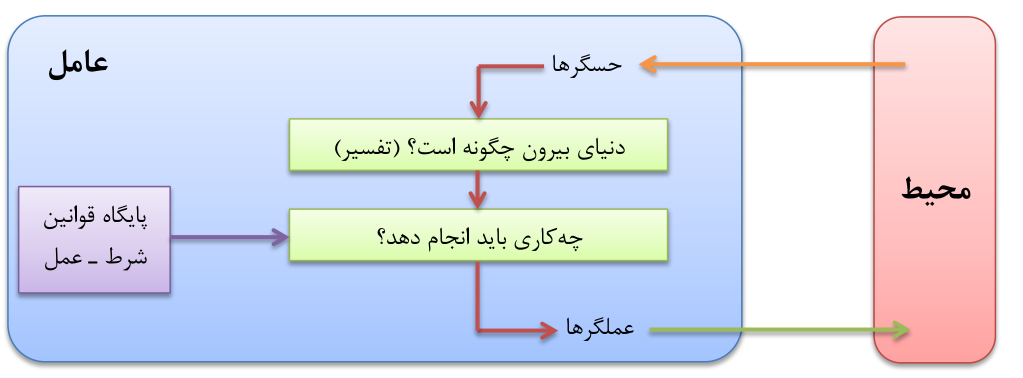
\includegraphics[scale=0.6]{./Untitled.png}
\end{center}


\vspace{20pt}
\noindent
عامل خودمختار چیست؟


\begin{tcolorbox}
\noindent
عامل های خود مختار : 

\noindent
عاملی خودمختار است که اکشن های آن بر اساس ادراکاتش اجرا شود . 

\noindent
خود مختاری وقتی که اکشن ها توسط ما به عملگر ها داده شوند از درجه ی پایین تری برخوردار است .

\noindent
عاملی که بر اساس یادگیری خود عمل می کند درجه ی خود 
مختاری بالاتری دارد .
\end{tcolorbox}




\newpage
\vspace{20pt}
\noindent
عامل عقلانی چیست؟

\begin{tcolorbox}
\noindent
عامل که بر اساس اطلاعاتی که از سنسور دریافت می کند و اعمالی که می تواند انجام دهد و دانش داخلی اش همواره بتواند کاری را انجام دهد که در راه رسیدن به هدف بیشترین موفقیت را کسب کند .

\end{tcolorbox}


\vspace{20pt}
\noindent
عقلانیت در یک عامل به چه چیزهایی بستگی دارد؟




\begin{tcolorbox}
\noindent
برای دستیابی به عقلانیت چهار فاکتور زیر باید به درستی تعریف شود :

\begin{enumerate}
	\item معیار کارایی
	\item دانش اولیه محیطی
	\item اعمال
	\item رشته ادراکات
\end{enumerate}
\end{tcolorbox}


\begin{latin}
\begin{tcolorbox}
\noindent
What is rational at any given time depends on four things:

\begin{enumerate}
	\item The \textbf{performance measure} that defines the criterion of success.
	\item The agent’s prior \textbf{knowledge of the environment.}
	\item The \textbf{actions} that the agent can perform.
	\item The agent’s \textbf{percept sequence} to date.
\end{enumerate}
\end{tcolorbox}
\end{latin}




\newpage
\vspace{20pt}
\noindent
قابلیتهای مورد نیاز سیستم تورینگ را بیان کنید.



\begin{tcolorbox}
آزمون تورینگ به این صورت انجام می‌گیرد که یک شخص به عنوان آزمایشگر، با یک ماشین و یک انسان به گفتگو می‌نشیند، و سعی در تشخیص ماشین از انسان دارد. در صورتی که ماشین بتواند قاضی را به گونه‌ای بفریبد که در قضاوت خود دچار اشتباه شود، توانسته‌ است آزمون را با موفقیت پشت سر بگذارد. برای اینکه تمرکز آزمون بر روی هوشمندی ماشین باشد، و نه توانایی آن در تقلید صدای انسان، مکالمه تنها از طریق متن و صفحه کلید و نمایشگر کامپیوتر صورت می‌گیرد. 
\end{tcolorbox}

\begin{tcolorbox}
\begin{itemize}
	\item پردازش زبان طبیعی 
	\item بازنمایی دانش 
	\item استدلال خودکار 
	\item یادگیری ماشینی 
\end{itemize}
\end{tcolorbox}


\begin{latin}
\begin{tcolorbox}
\begin{itemize}
	\item \textbf{natural language processing} to enable it to communicate successfully in English
	\item \textbf{knowledge representation} to store what it knows or hears
	\item \textbf{automated reasoning} to use the stored information to answer questions and to draw
new conclusions
	\item \textbf{machine learning} to adapt to new circumstances and to detect and extrapolate patterns.
\end{itemize}
\end{tcolorbox}
\end{latin}





\newpage
\vspace{20pt}
\noindent
گراف فضای حالت برای مساله جاروبرقی در فضای
 \lr{1x2}
 را رسم کنید.



\begin{center}
	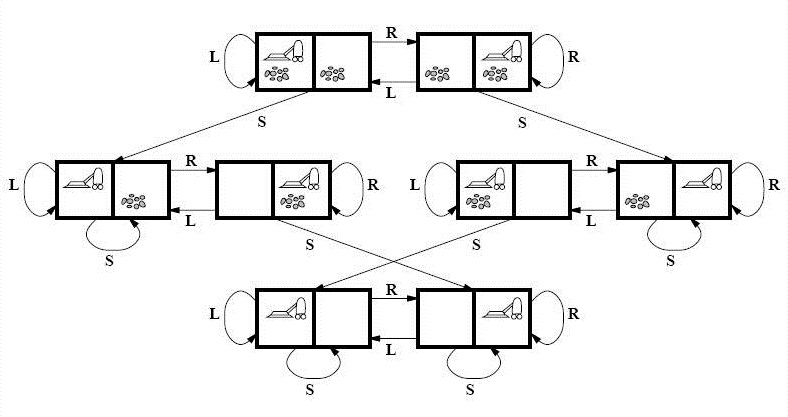
\includegraphics[scale=0.8]{./The-state-space-of-the-Vacuum-World-domain.jpg}
\end{center}




\vspace{20pt}
\noindent
معیارهای ارزیابی کارایی الگوریتم های جستجو را بیان کنید.



\begin{tcolorbox}
\noindent
برای بررسی الگوریتم های جستجو 4 معیار تعریف می شود :


\vspace{10pt}


\noindent
کامل بودن 
\lr{(Completeness)} :

\noindent
اگر مسئله ای دارای جواب باشد و الگوریتم جستجوی مورد نظر همیشه بتواند آنرا پیدا کند به آن الگوریتم کامل می گوییم .


\vspace{10pt}


\noindent
بهینه بودن 
\lr{(Optimality)} :

\noindent
اگر در مسئله ای بیش از یک مسیر به جواب وجود داشته باشد و یا دو جواب متفاوت وجود داشته باشد . الگوریتمی بهتر است که هزینه ی مسیری کمتری داشته باشد .



\vspace{10pt}


\noindent
پیچیدگی زمانی 
\lr{(Time Complexity)} :

\noindent
تعداد گره های تولید شده تا رسیدن به جواب ، پیچیدگی زمانی در نظر گرفته می شود .



\vspace{10pt}


\noindent
پیچیدگی مکانی 
\lr{(Space Complexity)} :

\noindent
میزان حافظه ی مورد نیاز برای رسیدن به جواب .

\end{tcolorbox}





\vspace{20pt}
\noindent
منظور از کامل بودن یک الگوریتم جستجو چیست؟



\begin{tcolorbox}
اگر مسئله ای دارای جواب باشد و الگوریتم جستجوی مورد نظر همیشه بتواند آنرا پیدا کند ، به آن الگوریتم ، الگوریتم کامل می گویند .
\end{tcolorbox}


\vspace{20pt}
\noindent
منظور از محیط پویا چیست؟ مثال بزنید.



\begin{tcolorbox}
\noindent
اگر در مدت سنجش محیط توسط عامل و اتخاذ تصمیم لازم ، محیط هیچ تغییری نکند ، آنگاه محیط ایستا است . در غیر این صورت محیط پویا است .

\noindent
محیط های نیمه پویا :

\noindent
محیط ذاتاً ایستا است اما با گذشت زمان معیار کارایی عامل تغییر پیدا کند . مثال : بازی شطرنج با ساعت .
\end{tcolorbox}


\vspace{20pt}
\noindent
منظور از محیط قطعی چیست؟ مثال بزنید.


\begin{tcolorbox}
\noindent
اگر در یک محیط حالت فعلی مشخص باشد ، با مشخص شدن عملی که می خواهیم انجام دهیم ، حالت بعدی محیط به صورت قطع معین خواهد شد ، به این محیط ، محیط قطعی یا معین گویند .

\vspace{20pt}
یا
\vspace{20pt}

\noindent
قطعی
\lr{(Deterministic)} :
	حالت بعدی مساله از روی وضعیت فعلی و عملی که می خواهیم انجام دهیم قابل شناسایی باشد .
	
\end{tcolorbox}





\newpage
\vspace{20pt}
\noindent
منظور از جستجوی ناآگاهانه چیست؟




\begin{tcolorbox}
الگوریتم جستجوی ناآگاهانه به غیر از صورت مسئله ، هیچ گونه اطلاعات دیگری در رابطه با مسئله در اختیار ندارد .
\end{tcolorbox}


\vspace{20pt}
\noindent
نکته کلیدی الگوریتم های جستجوی آگاهانه چیست؟




\begin{tcolorbox}
الگوریتم های جستجوی آگاهانه علاوه بر صورت مسئله ، اطلاعات بیشتری در رابطه با مسئله دارد .


نگرش کلی جستجو های آگاهانه انتخاب اولین-بهترین 
\lr{(Best-First)}
بر اساس تابع ارزیابی است .
\end{tcolorbox}


\begin{tcolorbox}
نکته ی کلیدی الگوریتم های جستجو ی آگاهانه استفاده از تابع هیوریستیک می باشد .
\end{tcolorbox}



\vspace{20pt}
\noindent
تفاوت الگوریتم های جستجوی ناآگاهانه و آگاهانه چیست؟


\begin{tcolorbox}
\textbf{ روش جستجو ناآگاهانه }
 روشی است که هیچ اطلاعات اضافی در باره ی نودهایی که قرار است بررسی کند نداشته باشد تا بتواند تصمیم بگیرد که ابتدا کدام نود را بررسی نماید
 
 \textbf{ روش جستجوی آگاهانه }
 یا مکاشفه‌ای از دانش مسئله استفاده می‌کند و نودی را انتخاب می‌کند که شانس رسیدن به هدف در آن بیشتر باشد یا به نظر آید که به هدف نزدیک تر است . برای اینکه تخمین بزنیم که نود فرزند چقدر به هدف نزدیک تر است از تابع ارزیابی استفاده می‌کنیم. این تابع هزینه رسیدن به نود هدف را تخمین می‌زند و به عبارت دیگر میزان مفید بودن نود فعلی را بازمی‌گرداند. 
\end{tcolorbox}






\newpage
\vspace{20pt}
\noindent
سه روش از روشهای رسمی تولید 
\lr{heuristic}
 را بنویسید. برای هر مورد یک مثال کوچک بزنید.




\begin{tcolorbox}
\begin{itemize}
	\item روش تجزیه: در این روش ، مسئله به مسئله‌های کوچکتر شکسته می‌شود که حل آن‌ها ساده‌تر است.
	\item روش استقرائی: در این نوع هیوریستیک‌ها سعی می‌شود راه‌حل به دست آمده برای مسئله در حالت ساده یا مقیاس کوچکتر، به مسئله اصلی تعمیم داده شود.
	\item روش تقلیل: در این روش‌  ، هدف، کاهش فضای راه‌حل‌های ممکن برای مسئله است. باید توجه داشت که در این صورت به علت حذف بخش قابل توجهی از فضای حالت ممکن است بعضی از جواب‌های بهینه نیز از دست بروند و در نهایت جواب شبه بهینه به دست آید یا اصلا جواب شبه بهینه‌ای برای مسئله پیدا نشود.
	\item روش سازنده: در این روش راه‌حل مسئله قدم به قدم و از صفر ساخته می‌شود. معمولاً راه‌حل‌های این دسته جزو الگوریتم‌های قطعی می‌باشند و به‌طور گسترده در بهینه‌سازی ترکیبیاتی استفاده می‌شوند.
\end{itemize}
\end{tcolorbox}





\newpage
\vspace{20pt}
\noindent
در مورد الگوریتمهای جستجوی 
\lr{(BFS- DFS- DLS- IDS)}
کدام یک کامل هستند و کدام یک کامل نیستند. دلیل خود را به طور واضح بیان نمایید.






\begin{tcolorbox}
الگوریتم 
 \lr{BFS} : 
 
 در این الگوریتم ابتدا نود ریشه بسط داده می شود ، سپس همه ی نود های فرزند ریشه بسط داده می شوند و سپس فرزندان آنها سطر به سطر بسط داده می شود .
 
 در این الگوریتم ابتدا تمامی نود ها در عمق 
 \lr{d}
 و سپس همه ی نودها  در عمق
 \lr{d+1}
 بسط داده می شوند .
 
 این الگوریتم کامل است چون جواب را پیدا می کند .
 
 \vspace{20pt}
 
 الگوریتم
  \lr{DFS} : 
  
  در این الگوریتم نودی که عمق بیشتری داشته باشد گسترش پیدا می کند ، اگر عمق گره ها یکی باشد ، گره ای که زودتر تولید شده گسترش پیدا می کند .
  
  الگوریتم 
   \lr{DFS}
   فقط یک مسیر از نود ریشه تا برگ را بررسی می کند 
   الگوریتم
   
   
   در صورتیکه زیر درخت سمت چپ عمق نامحدود داشته باشد و شامل هدف نباشد ، آنگاه این الگوریتم کامل نیست .
   
   
  \lr{DLS} : 
  
  جستجو با عمق محدود ، مشکل جستجو با عمق محدود را حل می کند .
  
  این جستجو ، درخت جستجو را از عمق
  \lr{L}
  به بعد حذف می کند .
  
  در صورتی که عمق هدف از 
  \lr{L}
  بیشتر باشد الگوریتم کامل نیست .
  
  
   الگوریتم
  \lr{IDS} : 
  
  این الگوریتم کامل و بهینه است .

\end{tcolorbox}









\end{document}




